\documentclass[12pt]{beamer}
\usepackage{graphicx}
\usepackage{nicefrac}
\usetheme{Warsaw}

\usepackage{tikz}
\usepackage{tkz-euclide} % loads  TikZ and tkz-base
\usetkzobj{all}
\title[]{EE2227}
\subtitle{Control Systems}

\institute{IIT HYDERABAD}
\author{Ganraj Borade(EE18BTECH11016)}

\date{}

\begin{document}


\begin{frame}
\titlepage
\end{frame}

\begin{frame}{Question no.13 from GATE/IN-2018}
An input p(t) = sin(t) is applied to the system $G(s) = \frac{s-1}{s+1} $. The corresponding steady state output is y(t) = sin(t + $\varphi$), where the phase $\varphi$ (in degrees), when restricted to 0$^{\circ}$ $\leq$ $\varphi$ $\leq$ 360$^{\circ}$, is ?



\end{frame}


 


\begin{frame}{Solution}

\vspace{4 mm}
We have p(t) = sin(t)

\vspace{4 mm}
We know that Laplace Transform of p(t) = $\mathcal{L}$(p(t)) = P(s)

\vspace{2 mm}
So , P(s) = $\frac{1}{s^2 + 1}$

\vspace{4 mm}

And we are given the steady state output $y_s(t)$ = sin(t+$\varphi$) 

\vspace{4 mm}
So , y_s(t) = sin(t)cos($\varphi$) + cos(t)sin($\varphi$) , 

\vspace{4 mm}
 Hence Laplace transform of y(t) in steady state = $\mathcal{L}$(y_s(t)) = Y_s(s) = \mathcal{L}(sin(t))cos($\varphi$) + $\mathcal{L}$(cos(t))sin($\varphi$)
 
\end{frame}

\begin{frame}
\vspace{4 mm}
Since , $\mathcal{L}$(sin(t)) = $\frac{1}{s^2 + 1}$ And $\mathcal{L}$(cos(t)) = $\frac{s}{s^2 + 1}$

\vspace{4 mm}
So , Y_s(s) = \frac{cos\varphi + s(sin\varphi)}{s^2 + 1} 

\vspace{4 mm}
And G(s) = $\frac{s-1}{s+1}$

\vspace{4 mm}
Hence , the output of the system in s-domain is Y(s) = P(s)G(s) 

\vspace{4 mm}
So , Y(s) = $\frac{1}{s^2 + 1}$ . $\frac{s-1}{s+1}$ , For solving this we can use the partial fractions :

\end{frame}

\begin{frame}
\vspace{4 mm}

Y(s) = $\frac{As + B}{s^2 + 1}$ + $\frac{C}{s + 1}$ = $\frac{(A+C)s^2 + (A+B)s + (B+C)}{(s^2 + 1)(s + 1)}$  

\vspace{4 mm}
Hence , by comparing coefficients ,

\vspace{4 mm }
we get A+C = 0 , A+B = 1 , B+C = -1

\vspace{4 mm}
After solving these above equations , we get A = 1 , B = 0 , C = -1. 

\vspace{4 mm}
So , Y(s) =  $\frac{s}{s^2 + 1}$ - $\frac{1}{s + 1}$

\vspace{4 mm}
Now we know that Laplace transform of e^{-t}u(t) = \mathcal{L}(e^{-t}u(t)) = \frac{1}{s+1}
\end{frame}

\begin{frame}
\vspace{4 mm}
i.e $\mathcal{L}$^{-1}(\frac{1}{s+1}) = e^{-1}u(t)


\vspace{4 mm}
 As for steady state analysis , we put t $\rightarrow$ $\infty$ ,therefore $e^{-1}u(t)$ will disappear while taking inverse laplace transform . Hence in steady state , only $\frac{s}{s^2 + 1}$ term will appear in laplace transform of y(t) as t $\rightarrow$ $\infty$

\vspace{4 mm}
Hence , in steady state , Y(s) = $\frac{s}{s^2 + 1}$ = $Y_s(s)$ given previously.

\vspace{4 mm}
So , $\frac{s}{s^2 + 1}$ = $\frac{cos(\varphi) + s(cos(\varphi))}{s^2 + 1}$

\vspace{4 mm}
By comparing coefficients of s and constants , we get $cos(\varphi)$ = 0 and $sin(\varphi)$ = 1 

\vspace{4 mm}

 

 So, because 0$^{\circ}$ $\leq$ $\varphi$ $\leq$ 360$^{\circ}$ , therefore $\varphi$ = 90$^{\circ}$


\end{frame}

\begin{frame}{}

Plot obtained for verification in python :
\setlength{\parindent}{1cm}
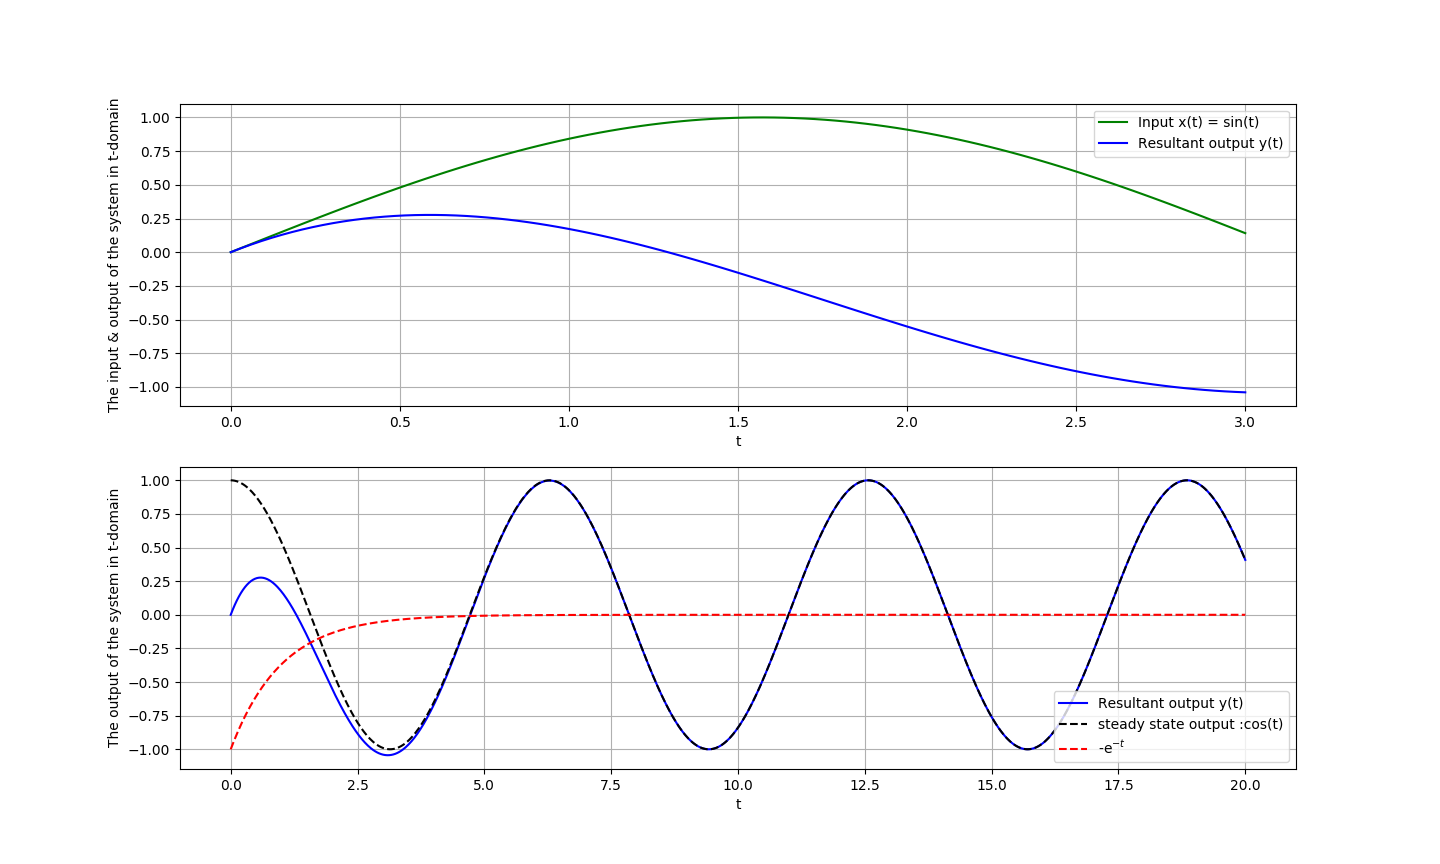
\includegraphics[scale=0.32, angle=0]{Figure_1.png}



\end{frame}
\begin{frame}
In above plot , black color plot is of cos(t).And blue color plot is the plot of resultant y(t) .So , we can see from above plots that black and blue color plots are coinciding after t = 3 . Hence y(t) = sin(t + 90$^{\circ}$) in steady state.

\end{frame}
\end{document}